\documentclass[letterpaper,11pt,twoside]{article}
\usepackage[utf8]{inputenc}
\usepackage{amsmath,amsfonts,amssymb,amsthm,latexsym}
\usepackage[spanish,es-noshorthands]{babel}
\usepackage[T1]{fontenc}
\usepackage{lmodern}
\usepackage{graphicx,hyperref}
\usepackage{tikz,pgf}
\usepackage{multicol}
\usepackage{fancyhdr}
\usepackage{marvosym}
\usepackage[height=9.5in,width=7in]{geometry}
\usepackage{fancyhdr}
\pagestyle{fancy}
\fancyhead[LE]{\Email matematicas.german@gmail.com}
\fancyhead[RE]{\url{https://www.autistici.org/mathgerman}}
\fancyhead[RO]{\Email matematicas.german@gmail.com}
\fancyhead[LO]{\url{https://www.autistici.org/mathgerman}}

\author{Germ\'an Avenda\~no Ram\'irez~\thanks{Lic. Mat. U.D., M.Sc. U.N.}}
\title{\begin{minipage}{.2\textwidth}

\includegraphics[height=1.75cm]{Images/logo-colegio.png}\end{minipage}
\begin{minipage}{.55\textwidth}
\begin{center}
Animaplano 05\\
Matemáticas $9^{\circ}$
\end{center}
\end{minipage}\hfill
\begin{minipage}{.2\textwidth}

\includegraphics[height=1.75cm]{Images/logo-sed.png} 
\end{minipage}}
\date{}
\thispagestyle{plain}
\begin{document}
\maketitle
Nombre: \hrulefill Curso: \underline{\hspace*{44pt}} Fecha: \underline{\hspace*{2.5cm}}
\begin{multicols}{2}
Responda frente a cada item haciendo el procedimiento correspondiente y luego ubique su respuesta en el plano dispuesto para hacer el animaplano.
\section*{Cuestionario}
 \begin{enumerate}
 \item Abscisa del punto origen del plano cartesiano
 \item Resuelva $\sqrt{8}\times \sqrt{18}=$
 \item Halle: $\sqrt{-36}=\underline{\hspace*{10pt}}i$
 \item $(a+b)^{2}=a^{2}+b^{2}$, \qquad F=18, \; V=38
 \item Si $a=b=c$, $abc=c^{3}$, \qquad V=29, \; F=15
 \item Si $4!+n=63$, entonces $n=$?
 \item El ancho de un rectángulo de área 3420 y su largo es 3 unidades más que su ancho.
 \item El quíntuplo del quinto número primo
 \item El décimo cuarto número primo
 \item El largo de un rectángulo cuya área es 1680 y su largo es 2 unidades más que su ancho.
 \item El largo de un rectángulo cuya área es 2550 y su ancho es 1 unidad menos que su largo.
 \item Vigésimo número primo
 \item $9^{2}+9^{0}=$
 \item $9^{2}+2(9^{0)}=$
 \item Halle $5!-(4!+3!)-(2^{2})^{2}$
 \item El triple de $5^{2}$
 \item $4^{2}\times 4=$
 \item El área de un rectángulo cuyo perímetro es 46 y cuyo largo es 15 unidades más que su ancho.
 \item El quíntuple del sexto número primo
 \item Encuentre el número $n$ que debe ir en: 136(47)230, \qquad 160($n$)314
 \item El área de un triángulo rectángulo cuya base mide 13 y su altura 12
 \item $9^{2}+9^{1}=$
 \item Sume 2 al perímetro de un pentágono regular de lado 17
 \item El mayor número de 2 cifras
 \item Un número que al duplicarlo, es 1/3 del número 582
 \item El 34\% de 250
 \item $(-35i^{2})+(-25i^{2})+(-24i^{2})=$
 \item Si $\frac{3}{2}=\frac{n}{14}$, luego $(n\times 4)+9=$
 \item 1 siglo -- 1 lustro -- 3 años =
 \item Si $n^{0}\times 70=x$, entonces $x=$?
 \item El producto entre la raíz cuadrada de 25 y la raíz cuadrada 100
 \item Si $4k^{2}-4=12$, $\rightarrow$ $k^{4}+k^{4}=$?
 \item Número que sumado son su doble da 99
 \item Resuelva $(9i^{2})\times (5i^{2})=$
 \item La suma de dos número es 85 y el mayor es 9 unidades más que el menor. El número mayor es:
 \item De acuerdo al anterior item, el número menor es:
 \item $(3^{0}\times 3^{1}\times 3^{2})+3^{0}=$
 \item La séptima parte de 112
 \item 1/5 del número 110
 \item $[(3^{5}-3^{4})+(8^{2}+9^{2})]\times (0)=$
 \end{enumerate}
\section*{Animaplano}
\begin{tikzpicture}[scale=.75]
%%Animaplano (0,0)--(9,9)
 \fill (0,0) node[above]{0} circle (0.2ex);
 \fill (1,0) node[above]{1} circle (0.2ex);
 \fill (2,0) node[above]{2} circle (0.2ex);
 \fill (3,0) node[above]{3} circle (0.2ex);
 \fill (4,0) node[above]{4} circle (0.2ex);
 \fill (5,0) node[above]{5} circle (0.2ex);
 \fill (6,0) node[above]{6} circle (0.2ex);
 \fill (7,0) node[above]{7} circle (0.2ex);
 \fill (8,0) node[above]{8} circle (0.2ex);
 \fill (9,0) node[above]{9} circle (0.2ex);
 \fill (0,-1) node[left]{10} circle (0.2ex);
 \fill (1,-1) circle (0.2ex);
 \fill (2,-1) circle (0.2ex);
 \fill (3,-1) circle (0.2ex);
 \fill (4,-1) circle (0.2ex);
 \fill (5,-1) circle (0.2ex);
 \fill (6,-1) circle (0.2ex);
 \fill (7,-1) circle (0.2ex);
 \fill (8,-1) circle (0.2ex);
 \fill (9,-1) circle (0.2ex);
 \fill (0,-2) node[left]{20} circle (0.2ex);
 \fill (1,-2) circle (0.2ex);
 \fill (2,-2) circle (0.2ex);
 \fill (3,-2) circle (0.2ex);
 \fill (4,-2) circle (0.2ex);
 \fill (5,-2) circle (0.2ex);
 \fill (6,-2) circle (0.2ex);
 \fill (7,-2) circle (0.2ex);
 \fill (8,-2) circle (0.2ex);
 \fill (9,-2) circle (0.2ex);
 \fill (0,-3) node[left]{30} circle (0.2ex);
 \fill (1,-3) circle (0.2ex);
 \fill (2,-3) circle (0.2ex);
 \fill (3,-3) circle (0.2ex);
 \fill (4,-3) circle (0.2ex);
 \fill (5,-3) circle (0.2ex);
 \fill (6,-3) circle (0.2ex);
 \fill (7,-3) circle (0.2ex);
 \fill (8,-3) circle (0.2ex);
 \fill (9,-3) circle (0.2ex);
 \fill (0,-4) node[left]{40} circle (0.2ex);
 \fill (1,-4) circle (0.2ex);
 \fill (2,-4) circle (0.2ex);
 \fill (3,-4) circle (0.2ex);
 \fill (4,-4) circle (0.2ex);
 \fill (5,-4) circle (0.2ex);
 \fill (6,-4) circle (0.2ex);
 \fill (7,-4) circle (0.2ex);
 \fill (8,-4) circle (0.2ex);
 \fill (9,-4) node[right]{49} circle (0.2ex);
 \fill (0,-5) node[left]{50} circle (0.2ex);
 \fill (1,-5) circle (0.2ex);
 \fill (2,-5) circle (0.2ex);
 \fill (3,-5) circle (0.2ex);
 \fill (4,-5) circle (0.2ex);
 \fill (5,-5) circle (0.2ex);
 \fill (6,-5) circle (0.2ex);
 \fill (7,-5) circle (0.2ex);
 \fill (8,-5) circle (0.2ex);
 \fill (9,-5) circle (0.2ex);
 \fill (0,-6) node[left]{60} circle (0.2ex);
 \fill (1,-6) circle (0.2ex);
 \fill (2,-6) circle (0.2ex);
 \fill (3,-6) circle (0.2ex);
 \fill (4,-6) circle (0.2ex);
 \fill (5,-6) circle (0.2ex);
 \fill (6,-6) circle (0.2ex);
 \fill (7,-6) circle (0.2ex);
 \fill (8,-6) circle (0.2ex);
 \fill (9,-6) circle (0.2ex);
 \fill (0,-7) node[left]{70} circle (0.2ex);
 \fill (1,-7) circle (0.2ex);
 \fill (2,-7) circle (0.2ex);
 \fill (3,-7) circle (0.2ex);
 \fill (4,-7) circle (0.2ex);
 \fill (5,-7) circle (0.2ex);
 \fill (6,-7) circle (0.2ex);
 \fill (7,-7) circle (0.2ex);
 \fill (8,-7) circle (0.2ex);
 \fill (9,-7) circle (0.2ex);
 \fill (0,-8) node[left]{80} circle (0.2ex);
 \fill (1,-8) circle (0.2ex);
 \fill (2,-8) circle (0.2ex);
 \fill (3,-8) circle (0.2ex);
 \fill (4,-8) circle (0.2ex);
 \fill (5,-8) circle (0.2ex);
 \fill (6,-8) circle (0.2ex);
 \fill (7,-8) circle (0.2ex);
 \fill (8,-8) circle (0.2ex);
 \fill (9,-8) circle (0.2ex);
 \fill (0,-9) node[left]{90} circle (0.2ex);
 \fill (1,-9) circle (0.2ex);
 \fill (2,-9) circle (0.2ex);
 \fill (3,-9) circle (0.2ex);
 \fill (4,-9) circle (0.2ex);
 \fill (5,-9) circle (0.2ex);
 \fill (6,-9) circle (0.2ex);
 \fill (7,-9) circle (0.2ex);
 \fill (8,-9) circle (0.2ex);
 \fill (9,-9) node[right]{99} circle (0.2ex);
% \draw (0,0)--(2,-1)--(6,0)--(8,-1)--(9,-2)--(9,-3)--(7,-5)--(5,-5)--(3,-4)--(2,-4)--(1,-5)--(1,-7)--(2,-8)--(3,-8)--(4,-7)--(5,-7)--(4,-6)--(6,-7)--(5,-6)--(7,-7)--(8,-7)--(9,-8)--(7,-8)--(9,-9)--(7,-9)--(5,-8)--(4,-8)--(3,-9)--(2,-9)--(0,-7)--(0,-5)--(2,-3)--(3,-3)--(5,-4)--(7,-4)--(8,-3)--(8,-2)--(6,-1)--(2,-2)--(0,0);
\end{tikzpicture}
\section*{Preparándonos para las pruebas saber}
Responda las preguntas \ref{q01}--\ref{q02} de acuerdo con la siguiente información

Se les preguntó a 32 estudiantes de un colegio por el número de horas que dedican a ver televisión diariamente. Los resultados aparecen en la siguiente lista.
\begin{center}
0, 2, 4, 2, 2, 2, 2, 3, 3, 4, 0, 2, 4, 2, 2, 4, 0, 4, 2, 2, 4, 2, 2, 3, 3, 2, 2, 2, 2, 4, 4, 0
\end{center}
\begin{enumerate}
\item ¿Cuál es la moda de esta lista? \label{q01}
\begin{enumerate}
\begin{multicols}{4}
\item 0
\item 2
\item 3
\item 4
\end{multicols}
\end{enumerate}
\item ¿En cuál de los siguientes diagramas circulares se representa correctamente la información de la lista? \label{q02}
\begin{center}
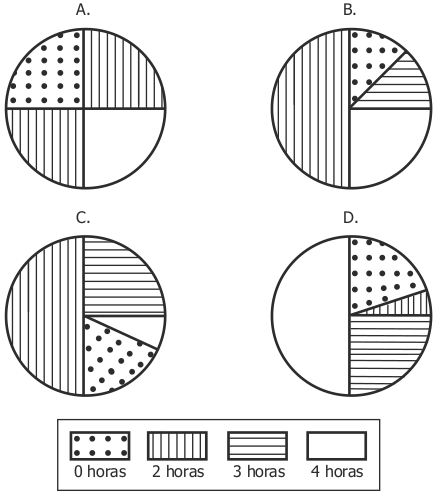
\includegraphics[scale=.5]{Images/Pantallazo-12.png} 
\end{center}
\item La figura 1 muestra la temperatura ambiente de un lugar a las 5:00 de la mañana, la figura 2 muestra la temperatura ambiente del mismo lugar a la 1:00 de la tarde y la figura
3 muestra la temperatura ambiente del mismo lugar a las 6:00 de la tarde.
\begin{center}
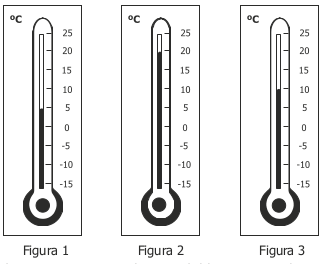
\includegraphics[scale=.7]{Images/Pantallazo-13.png} 
\end{center}
¿Cuál fue el cambio de temperatura ambiente del lugar entre las 5:00 de la mañana y las 6:00 de la tarde?
\begin{enumerate}
\item Disminuyó 15$^{\circ}C $
\item Disminuyó en 10$^{\circ}C$
\item Aumentó 5$^{\circ}C$
\item Aumentó 20$^{\circ}C$
\end{enumerate}
\end{enumerate}
\end{multicols}
\end{document}
